\documentclass{article}
\usepackage{amsmath}
\usepackage{graphicx}
\usepackage{apacite}  

\setlength\parindent{24pt}
% Keywords command
\providecommand{\keywords}[1]
{
  \small	
  \textbf{\textit{Keywords---}} #1
}

\title{\textbf{Evaluating KNN, SVR, ANN, XGBoost Regressor, Linear Regression, and Random Forest Models for Dengue Case Prediction: A Comparative Study}}
\author{
    Kurt Matthew Amodia \and 
    Glen Andrew Bulaong \and 
    Carl Benedict Elipan \and 
    John Hamir Karim
}
\date{}

\begin{document}
\maketitle

\begin{abstract}
Dengue fever remains a pressing public health challenge in the Philippines, with cases rising significantly in recent years. In Iloilo City, the Iloilo Provincial Health Office reported a sharp increase in dengue cases, from 1,095 cases and one fatality in 2022 to 4,585 cases and 10 fatalities as of August 10, 2023—a 319\% year-on-year surge. To address this, machine learning algorithms offer promising tools for predicting dengue outbreaks and informing timely interventions. This study analyzes dengue data from the Iloilo Provincial Health Office and climate data from online sources, using six machine learning algorithms: K-Nearest Neighbors (KNN), Linear Regression, Support Vector Regression (SVR), Random Forest, Artificial Neural Network (ANN), and XGBoost Regression. Running these algorithms on the dataset through the Scikit-learn Python library, results indicate that Random Forest performed best for dengue prediction, with an RMSE of 25.4081 and MAE of 16.7267, while KNN emerged as the least effective, with an RMSE of 48.4247 and MAE of 25.7855. These findings underscore the potential of advanced machine learning models in improving dengue forecasting and enhancing public health responses in Iloilo City.

\keywords{K-Nearest Neighbors (KNN), Linear Regression, Support Vector Regression (SVR), Random Forest, Artificial Neural Network (ANN), and XGBoost Regression, Machine learning, Dengue forecasting }
\end{abstract}

\section{Introduction}

From 2020 to 2022, dengue cases declined due to reduced surveillance during the COVID-19 pandemic \cite{WHO2023}, but cases surged in 2023 as restrictions were lifted. This year saw an increase in dengue outbreaks worldwide, with over five million cases and more than 5,000 deaths reported in over 80 countries \cite{bosano2023who}. Dengue is endemic in the Philippines, leading to longer and more widespread seasonal outbreaks. Globally, dengue infections have increased significantly, posing a major public health challenge. 

The World Health Organization reported a ten-fold rise in cases between 2000 and 2019, with a peak in 2019 when the disease spread across 129 countries \cite{WHO2024}. Iloilo City and Province are intensifying efforts to curb the rising dengue cases \cite{lena2024}. As of August 10, 2023, the Iloilo Provincial Health Office recorded 4,585 cases and 10 deaths, a 319\% increase from last year’s 1,095 cases and one death. 

Governor Arthur Defensor Jr. confirmed that the province has reached the dengue outbreak threshold based on the Department of Health (DOH). Local government units (LGUs) have been informed, and the province’s disaster management office is on blue alert, indicating disaster mode. \cite{PNA2024} In Iloilo City, 649 dengue cases were recorded this year 2024, with two deaths. Cases cluster in 40 out of 180 barangays, meaning multiple cases are being reported in these areas over several weeks. The city’s health officer, Dr. Roland Jay Fortuna, reported high utilization of non-COVID-19 hospital beds, reaching over 76\%, prompting concerns about hospital capacity. 

This study aims to evaluate and compare six models—K-Nearest Neighbors (KNN), Linear Regression, Support Vector Regressor (SVR), Random Forest, Artificial Neural Network (ANN), and XGBoost Regressor  —in predicting dengue cases, with a focus on applicability in Iloilo City. Accurate prediction models are valuable in this context, as they provide health agencies with insights into expected case numbers, supporting proactive measures for outbreak control and resource allocation.

Specifically, this study aims to:
\begin{enumerate}
    \item Gather dengue data from the Iloilo Provincial Health Office and climate data from online sources. Combine these data into a unified dataset to facilitate comprehensive dengue case forecasting.
    \item Train and evaluate model metrics, including K-Nearest Neighbors (KNN), Linear Regression, Support Vector Regressor (SVR), Random Forest, Artificial Neural Network (ANN), and XGBoost Regressor for predicting dengue cases.
    \item Compare the performance of these models to determine the most accurate forecasting approach.
\end{enumerate}

\subsection{Literature Review}
Dengue prediction models have been extensively studied to improve outbreak forecasting and public health responses. A study in China utilized weekly dengue cases, climate factors, and Baidu search queries to develop predictive models using machine learning algorithms \cite{guo2017developing}. Among the models tested, Support Vector Regression (SVR) demonstrated superior performance, achieving the smallest prediction errors and accurately forecasting dengue outbreaks, including the peak of a major 2014 epidemic. The study highlighted the utility of SVR in capturing nonlinear relationships in time-series data, making it a robust tool for dengue forecasting across diverse regions.

Similarly, in Colombia, a national Random Forest model using historical dengue cases, environmental data, and sociodemographic variables outperformed local models and ANN models. The RF model's accuracy was higher for short-term forecasts, emphasizing environmental predictors, while sociodemographic factors gained importance for longer-term trends \cite{zhao2020machine}. This approach highlights the utility of RF models in dengue forecasting and the value of incorporating diverse predictors for both short- and long-term trends.

In Malaysia, dengue outbreaks in Selangor were modeled using climate variables such as temperature, wind speed, humidity, and rainfall. Among the models tested, the SVM with a linear kernel demonstrated the best prediction performance, with an accuracy of 70\% and improved sensitivity for balanced datasets \cite{salim2021prediction}. The study emphasized the "week-of-the-year" as a critical predictor, showcasing the potential of machine learning in managing dengue outbreaks. Future studies suggest exploring boosting techniques or nature-inspired algorithms to enhance model performance.

\section{Methodology}
This chapter lists and discusses the specific steps and activities that were performed to accomplish this mini-project.

\begin{figure}[h!]
    \centering
    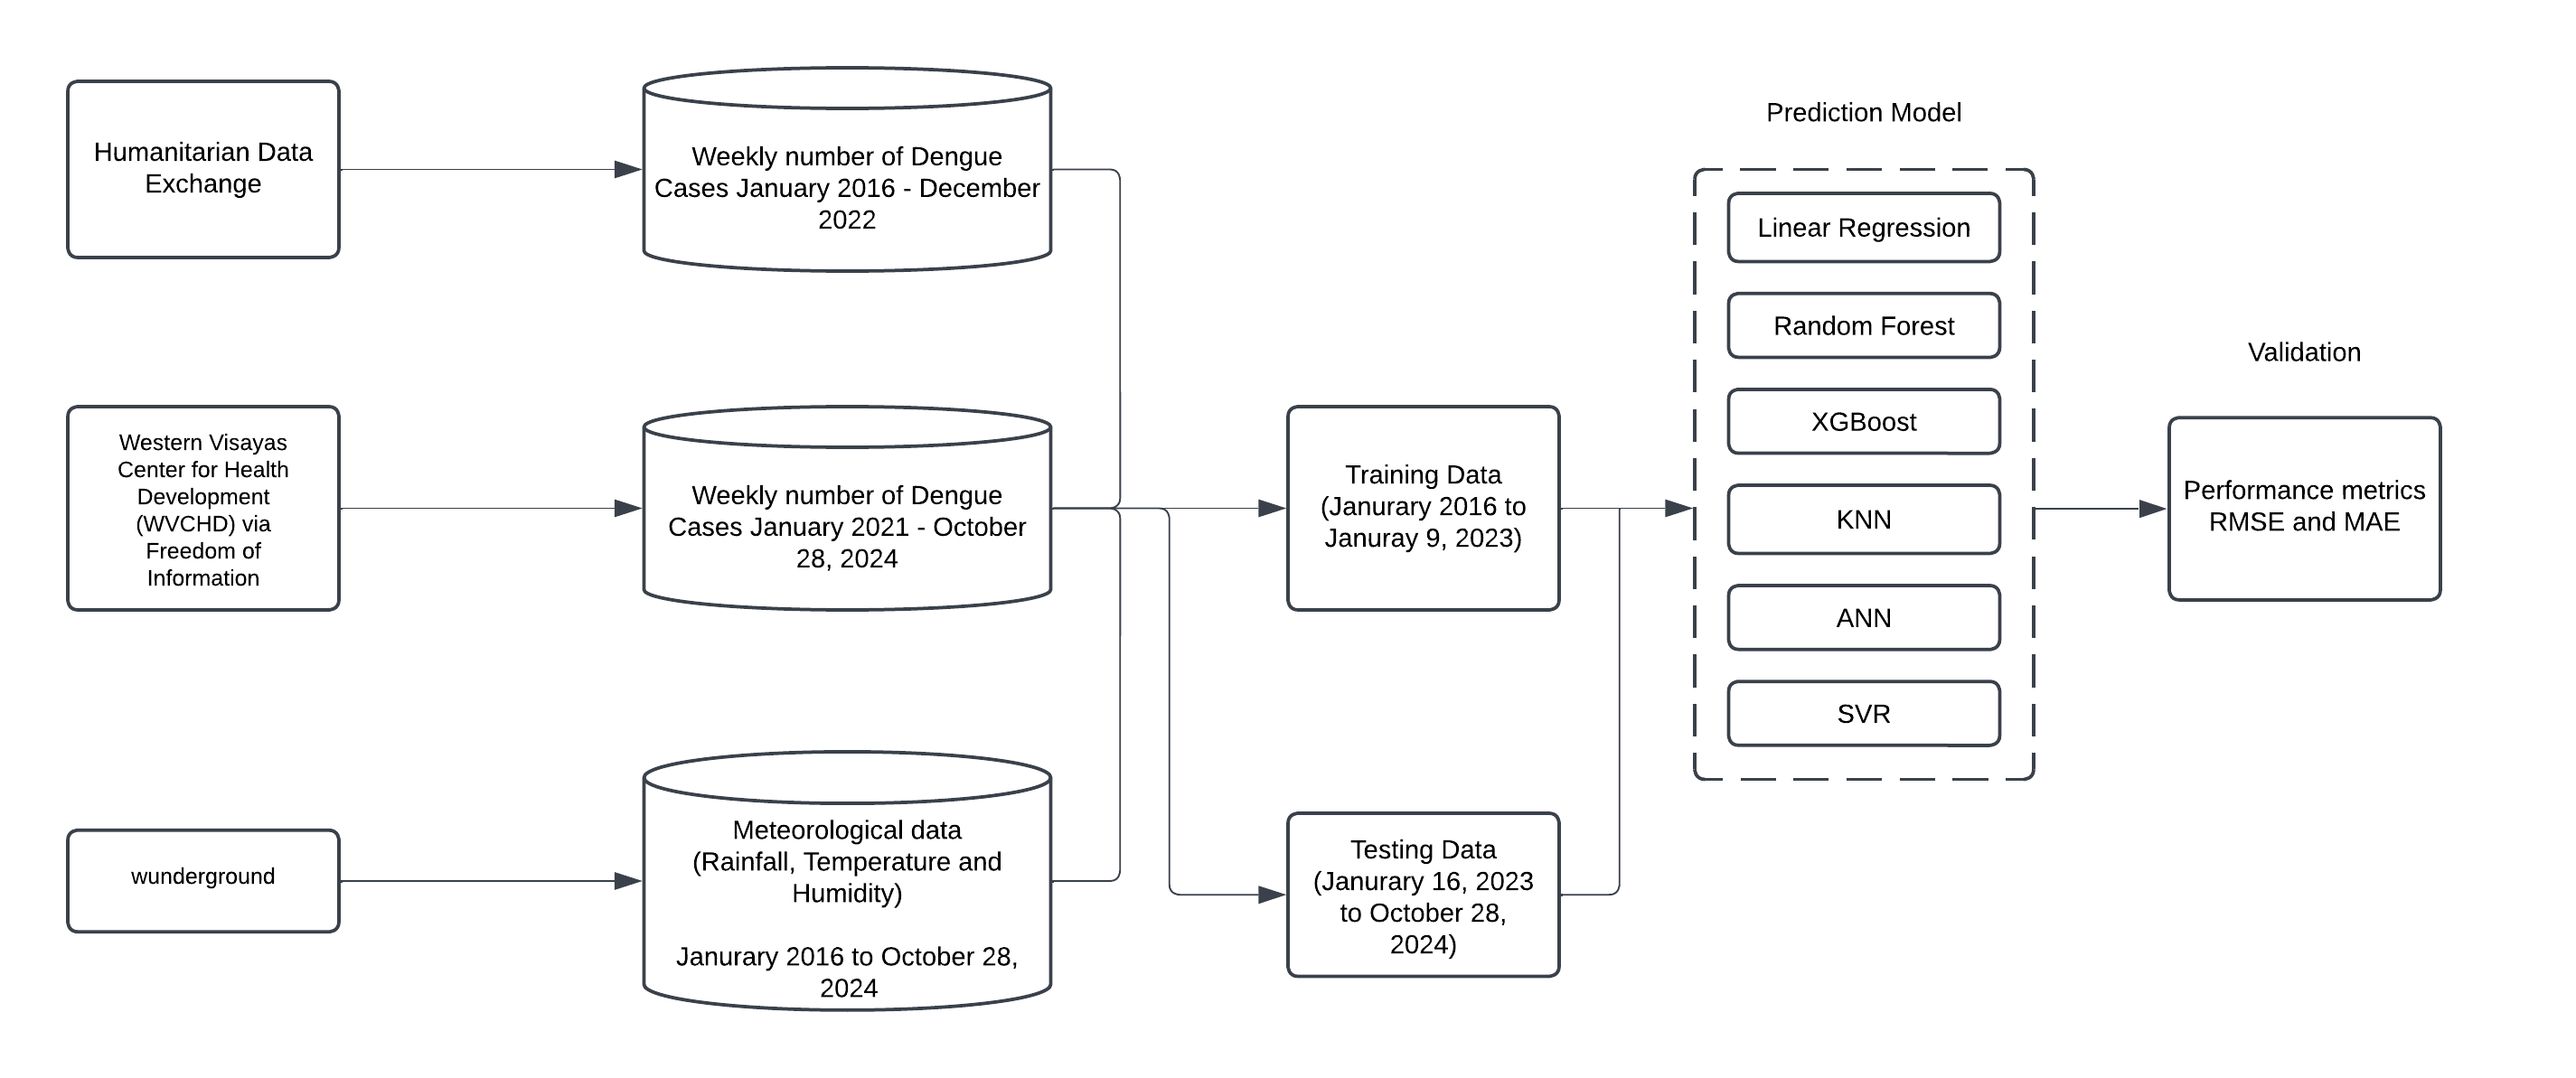
\includegraphics[width=1\linewidth]{image/Model Diagram.png}
    \caption{Workflow Diagram}
    \label{fig:workflow}
\end{figure}

In figure \ref{fig:workflow}. This summarizes the workflow done in the study. The approach involves deploying several models for prediction, including Artificial Neural Network (ANN), K-Nearest Neighbors (KNN), Linear Regression, Support Vector Regressor (SVR), Random Forest, and XGBoost. These machine-learning methods are then compared with each other to determine the most accurate model.

\subsection{Data}
\subsubsection{Acquisition of Dengue Case Data}
The historical dengue case dataset used in this study was obtained from the Humanitarian Data Exchange and the Western Visayas Center for Health Development (WVCHD) via Freedom of Information (FOI) requests. Also, the collection of weather data was done by utilizing web scraping techniques to extract weekly weather data (e.g., rainfall, temperature, and humidity) from Weather Underground (wunderground.com).
\\
\\
\textbf{Data Fields}
\begin{itemize}
    \item \textbf{Time.} Represents the specific year and week corresponding to each entry in the dataset.
    \item \textbf{Rainfall.} Denotes the observed average rainfall, measured in millimeters, for a specific week.
    \item \textbf{Humidity.} Refers to the observed average relative humidity, expressed as a percentage, for a specific week.    
    \item \textbf{Temperature.} Represents the observed average temperature, measured in degrees Celsius, for a specific week.
    \item \textbf{Cases.} Refers to the number of reported dengue cases during a specific week.
\end{itemize} 

\subsubsection{Data Integration and Preprocessing}
The dengue case data was integrated with the weather data to create a comprehensive dataset, aligning the data based on corresponding timeframes. The dataset undergoed a cleaning process to address any missing values, outliers, and inconsistencies to ensure its accuracy and reliability. To ensure that all features and the target variable were on the same scale, a MinMaxScaler was applied to normalize both the input features (rainfall, temperature, humidity) and the target variable (dengue cases). To enhance the quality of the data and minimize the impact of random short-term fluctuations, moving averages was applied to selected columns, including rainfall, humidity, and temperature. This approach will help to filter out 'noise' and provide a clearer representation of the underlying trends.

\subsection{Model Training}
The following models were selected and trained using the Scikit-learn Python library to forecast dengue cases based on historical weather and case data. The dataset will be split into training and testing sets, ensuring temporal continuity is maintained to avoid data leakage. All models are grid-searched in each specific hyperparameter, and each model was fine-tuned for optimal performance:

\subsubsection{KNN Model}
The number of neighbors (k) was set to 7, which was selected after experimentation with different values of k to ensure the best balance between bias and variance. KNN is a non-parametric algorithm that predicts the target variable based on the average of the k-nearest neighbors in the feature space. The model was trained using the normalized features and evaluated by comparing predicted and actual dengue cases.

\subsubsection{Support Vector Regression Model}
\textbf{Hyperparameters}
\begin{itemize}
    \item \textbf{C:} 100, which controls the penalty for misclassification. A higher value emphasizes correct classification at the cost of margin width.
    \item \textbf{Gamma:} 0.01, which defines how far the influence of a single training point reaches. Smaller values lead to a more generalized model.
    \item \textbf{Epsilon:} 0.02, which specifies the margin of tolerance where no penalty is given for errors.
\end{itemize}

\subsubsection{Artificial Neural Network}
The model was trained with a learning rate of 0.001, utilizing the Adam optimizer to ensure efficient training. The training process was set to run for 200 epochs, with a batch size of 16, meaning 16 training samples were processed per iteration. To capture complex patterns without overfitting, a hidden layer consisting of 64 neurons with a ReLU activation function was chosen. The architecture followed a Sequential Neural Network design, incorporating an input layer, one hidden layer, and an output layer. Additionally, early stopping was implemented to prevent overfitting by monitoring the validation performance during training.

\subsubsection{XGBoost Regressor Model}
The model was trained using XGBoost with the following hyperparameters: 200 boosting rounds to enhance model performance, and a learning rate of 0.05 to promote better generalization. The maximum depth of the decision trees was set to 6 to control overfitting, while the minimum child weight was set to 1 to regulate the minimum sum of instance weights in each child. To further prevent overfitting, subsample, and colsamplebytree were both set to 0.8, indicating that 80\% of the samples and features, respectively, were used for each tree. 

\subsubsection{Linear Regression}
No hyperparameter tuning was applied to the linear regression model, as it is a straightforward model with minimal tunable parameters. The model assumes a linear relationship between the input features and the target variable. Linear regression was chosen as a baseline model to predict dengue cases, relying on the linear correlation between weather variables and the target. 

\subsubsection{Random Forest Model}
The model was trained using Random Forest with the following hyperparameters: 100 estimators , indicating the number of decision trees in the forest, and a random state of 42 to ensure reproducibility of results. The model was trained using a normalized dataset and evaluated against the test set to assess its performance.

\subsection{Model Evaluation}
After training, the models were evaluated using three primary metrics to assess their performance:
\begin{itemize}
    \item \textbf{Mean Absolute Error (MAE):} Measures the average absolute differences between predicted and actual values.
    \item \textbf{Mean Squared Error (MSE):} Measures the average of the squares of the errors, giving more weight to larger errors.
    \item \textbf{Root Mean Squared Error (RMSE):} The square root of MSE, providing an interpretation in the original units of the target variable.
\end{itemize}

The predicted values for dengue cases were compared to the actual values, and performance metrics were calculated to assess each model's forecasting accuracy.

\subsection{Model Comparison}
The performance of each model was compared to determine the most accurate forecasting approach. A plot was generated to visually compare the actual versus predicted values of dengue cases for each model.

\pagebreak
\section{Results and Discussion}
\begin{table}[h!]
\centering
\begin{tabular}{||c | c | c | c||} 
 \hline
 \textbf{Model} & \textbf{MAE} & \textbf{RMSE} & \textbf{MSE} \\ [1ex] 
 \hline
 \textbf{KNN} & 25.7855 & 48.4247 & 2344.9568 \\ 
 \hline
 \textbf{SVR} & 15.3458 & 29.9683 & 898.0991 \\
 \hline
 \textbf{ANN} & 13.5304 & 27.3499 & 748.0170 \\
 \hline
 \textbf{XGBoost} & 18.8749 & 27.5577 & 759.4290 \\
 \hline
 \textbf{Linear Regression} & 16.3724 & 29.5676 & 874.2463 \\ 
 \hline
 \textbf{Random Forest} & 16.7267 & 25.4081 & 645.5732 \\ [1ex] 
 \hline
\end{tabular}
\caption{Summary of Results}
\label{table:summary}
\end{table}

\subsubsection{KNN Model}
The K-Nearest Neighbors (KNN) model achieved a Mean Absolute Error (MAE) of 25.7855, indicating that the average prediction deviates from the actual dengue cases by roughly 26 cases. The Mean Squared Error (MSE) of 2344.9568 suggests that the squared differences between actual and predicted cases are significantly large, primarily due to extreme deviations. The Root Mean Squared Error (RMSE) of 48.4247 further confirms this, reflecting considerable variability in the errors. This suggests that KNN's model could be struggling with larger deviations, making it less robust compared to others.
\begin{figure}[h!]
    \centering
    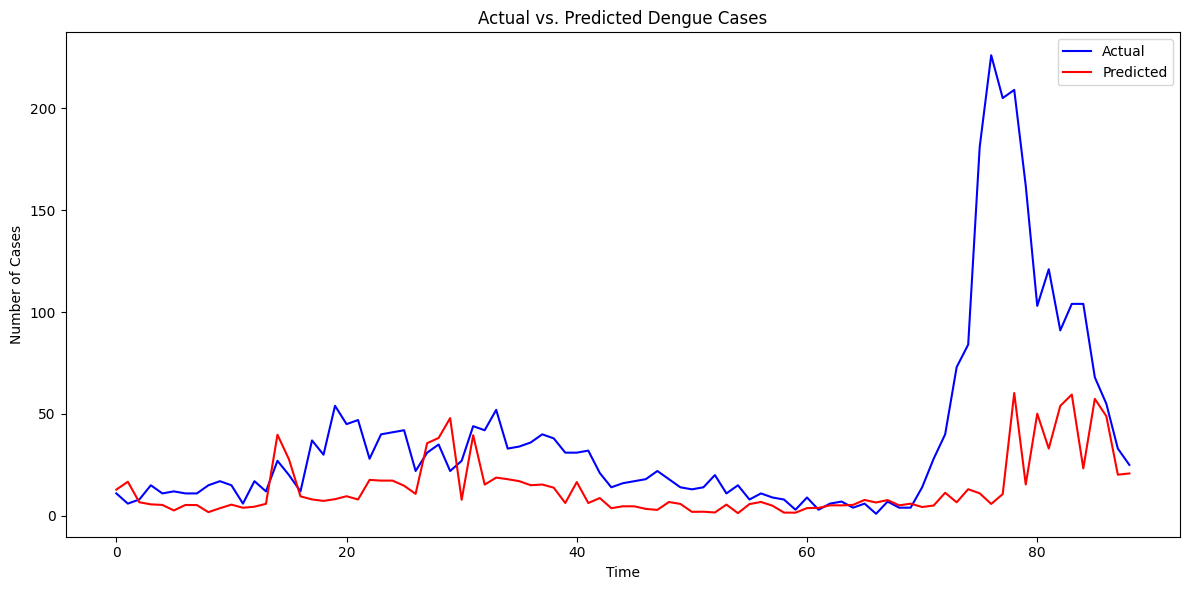
\includegraphics[width=1\linewidth]{image/knn plot.png}
    \caption{KNN Actual vs Predicted}
    \label{fig:knn}
\end{figure}

In Figure \ref{fig:knn}, the predicted values (red line) generally follow the trend of the actual cases (blue line) in some periods but fail to capture the exact magnitudes of the dengue cases. The model struggles to predict extreme increases and decreases in dengue cases, resulting in significant underestimation or overestimation during peaks. For instance, during periods of rapid increase or decrease, the model fails to reflect the true magnitude of changes. This limitation is likely due to KNN’s sensitivity to the nearest neighbors, which may not represent rare or extreme patterns effectively. While it captures overall patterns, the high variability in dengue cases poses a challenge for this model.

\subsubsection{SVR Model}
The Support Vector Regression (SVR) model shows an MAE of 15.3458, implying moderately accurate predictions with an average error of 15.35 cases. The MSE of 898.0991 and the RMSE of 29.9683 show improvement over KNN, with smaller squared errors and deviations.
\begin{figure}[h!]
    \centering
    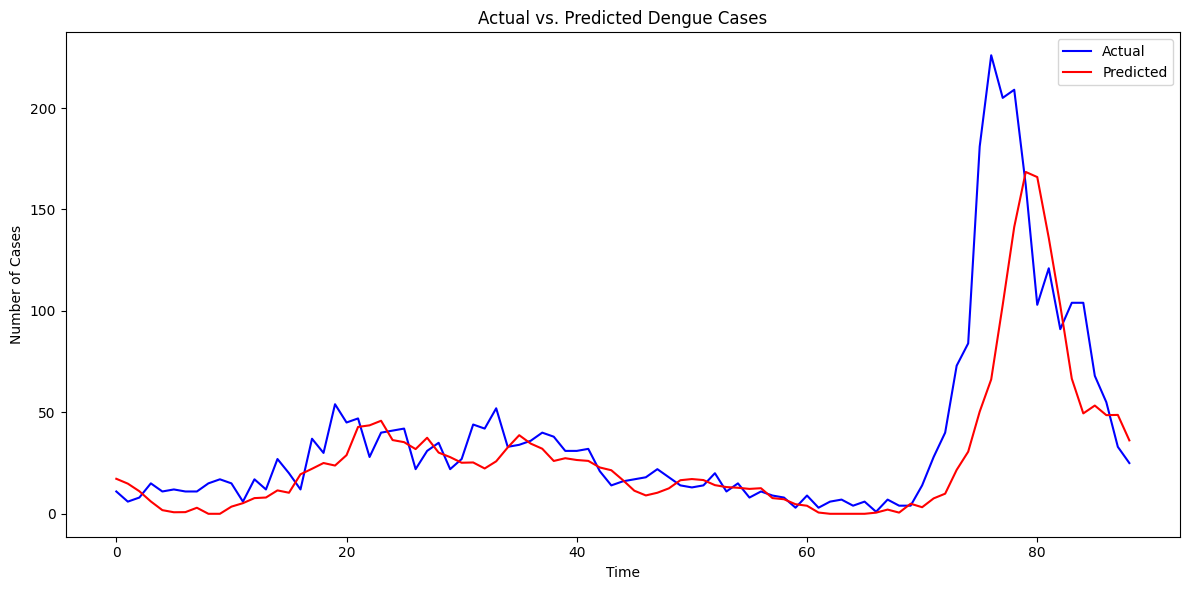
\includegraphics[width=1\linewidth]{image/svr plot.png}
    \caption{SVR Actual vs Predicted}
    \label{fig:svr}
\end{figure}

In Figure \ref{fig:svr}. Although the predicted values follow the trend of the actual values closely, The predicted values (red line) deviate significantly from the actual values (blue line) in high dengue case ranges. The model performs reasonably well in capturing overall trends in moderate ranges.

\subsubsection{ANN Model}
The ANN model has the lowest MAE, indicating that it generally makes more accurate predictions, with deviations around 13.53 units on average. The Mean Squared Error (MSE) of 748.0170 reveals notable variability between actual and predicted values, particularly at higher case counts. The Root Mean Squared Error (RMSE) of 27.3499 is also relatively low, suggesting that the model has fewer large errors compared to KNN.
\begin{figure}[h!]
    \centering
    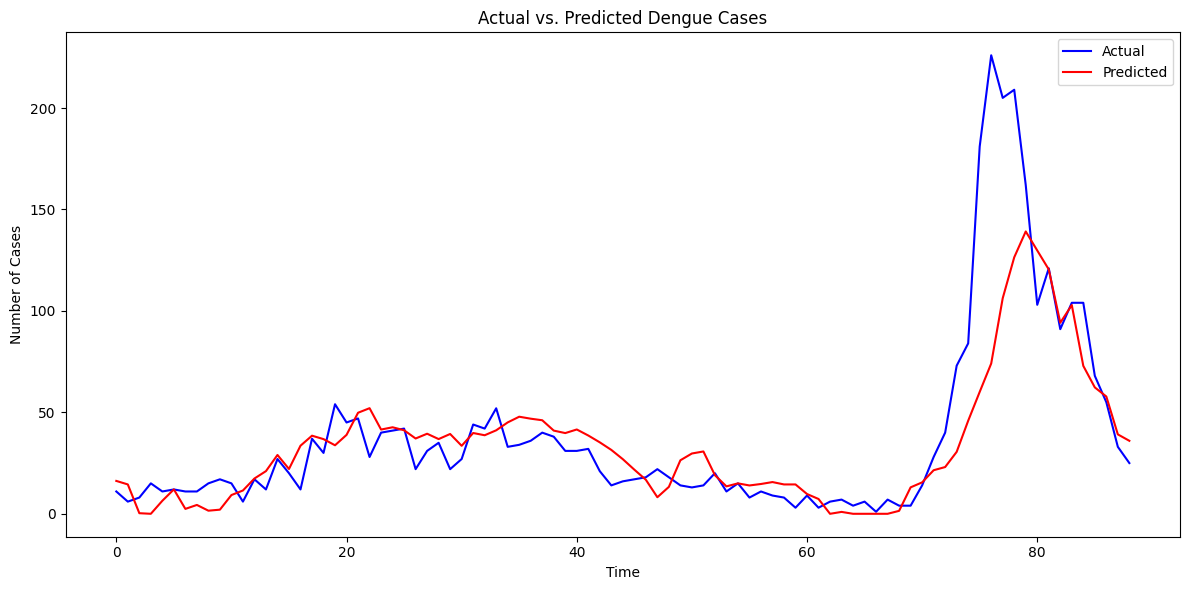
\includegraphics[width=1\linewidth]{image/Ann plot.png}
    \caption{ANN Actual vs Predicted}
    \label{fig:ann}
\end{figure}

In Figure \ref{fig:ann}. the ANN model aligns closely with the actual dengue case trends, particularly in low to moderate ranges. However, during extreme spikes, the model underestimates the actual values. This reflects the ANN’s strength in capturing nonlinear patterns due to its architecture, though it still faces challenges in modeling abrupt changes due to limited training data on such rare events.

\subsubsection{XGBoost Regressor Model}
The XGBoost model achieved an MAE of 18.8749, showing good accuracy in minimizing the average prediction errors. The MSE is 759.4290, indicating moderate variability in predictions. The RMSE of 27.5577 reflects that while the model performs well overall, it struggles slightly with outliers or extreme spikes in dengue cases.

\begin{figure}[h!]
    \centering
    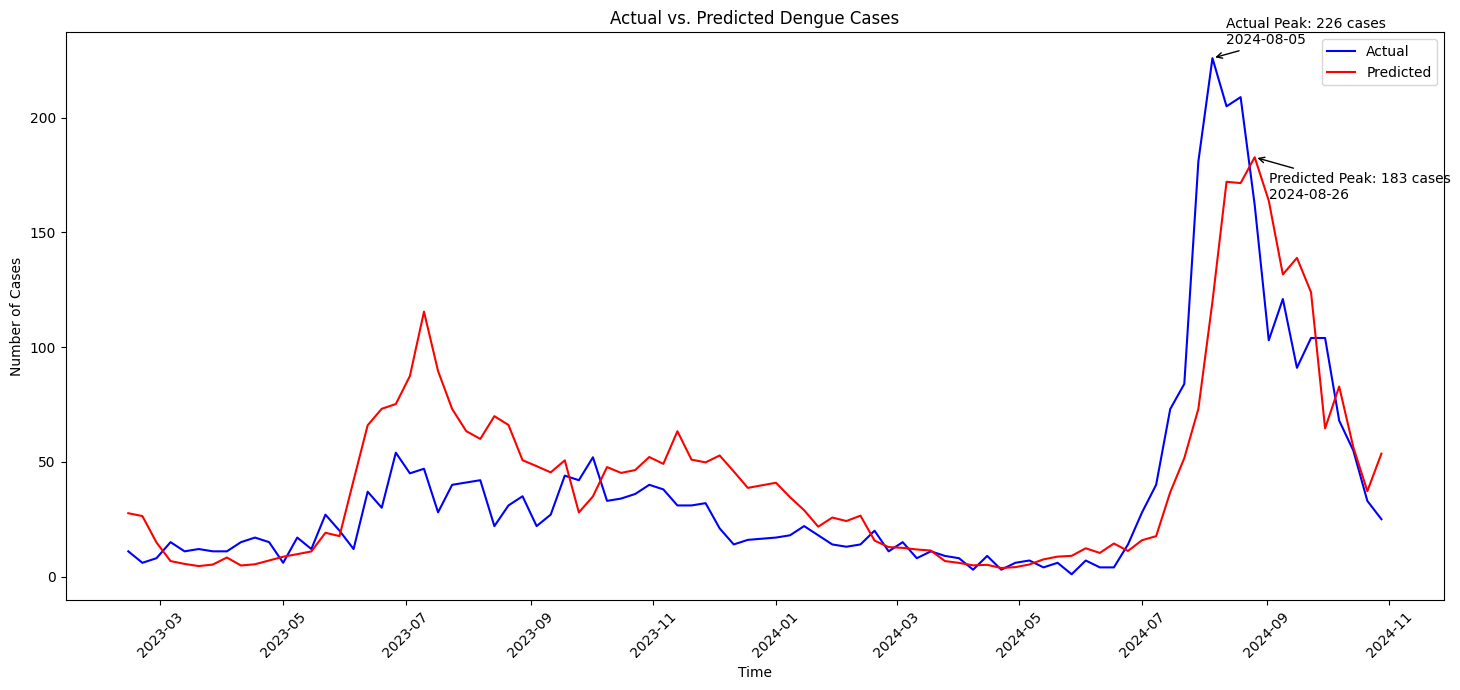
\includegraphics[width=1\linewidth]{image/XGBoost plot.png}
    \caption{XGBoost Actual vs Predicted}
    \label{fig:xgb}
\end{figure}

In Figure \ref{fig:xgb}. The XGBoost model effectively captures the overall trend of dengue case fluctuations. The model performs reliably in predicting low to moderate dengue cases, with a reasonable alignment between actual and predicted values for dengue cases. There is a slight overshooting however for small spikes in the dataset. The ensemble-based nature of XGBoost provides robustness and good generalization, though fine-tuning could potentially improve performance for extreme cases.

\subsubsection{Linear Regression Model}
The Linear Regression model achieved a Mean Absolute Error (MAE) of 16.3724, indicating a low average error and a high degree of accuracy. The Mean Squared Error (MSE) of 874.2463 suggests limited variability in predictions, demonstrating the model's strong ability to generalize across data. Additionally, the Root Mean Squared Error (RMSE) of 29.5676 highlights the model's robust performance, even when larger errors are penalized more significantly.\\

\begin{figure}[h!]
    \centering
    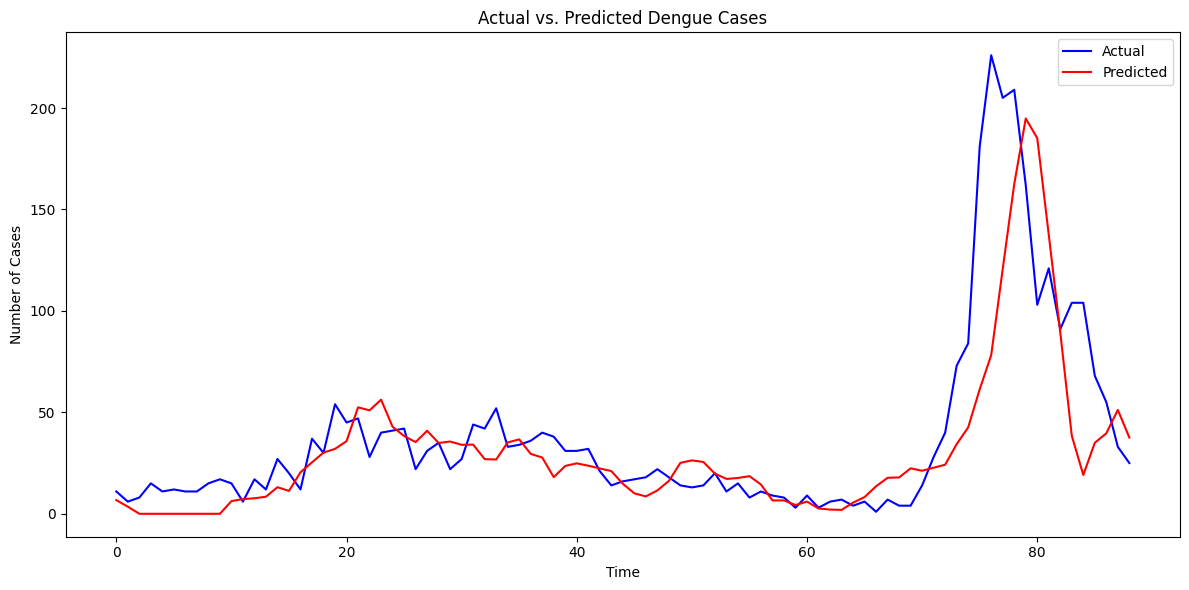
\includegraphics[width=1\linewidth]{image/Linear Regression plot.png}
    \caption{Linear Regression Actual vs Predicted}
    \label{fig:lr}
\end{figure}

Figure \ref{fig:lr}. shows that the predicted values (red) closely follow the trends of the actual values (blue), showcasing Linear Regression's capability to effectively capture patterns in low and moderate case ranges. Although slight deviations occur in high-peak regions, the model remains consistent and aligns well with the actual data. However, we have to keep in mind that the preprocessing techniques, such as moving averages, have helped reduce noise, allowing the model to focus on broader patterns effectively.

\subsubsection{Random Forest Model}
The Random Forest model achieved an MAE of 16.7267, indicating that, on average, its predictions are off by about 17 dengue cases. The MAE for Random Forest is relatively similar to that of linear regression, indicating moderate prediction accuracy, but still not as good as ANN. However, the MSE for Random Forest is the lowest, which indicates that its predictions are relatively close to the actual values, with fewer extreme errors. Random Forest has a lower RMSE than any other model, showing fewer large errors compared to the other models.


\begin{figure}[h!]
    \centering
    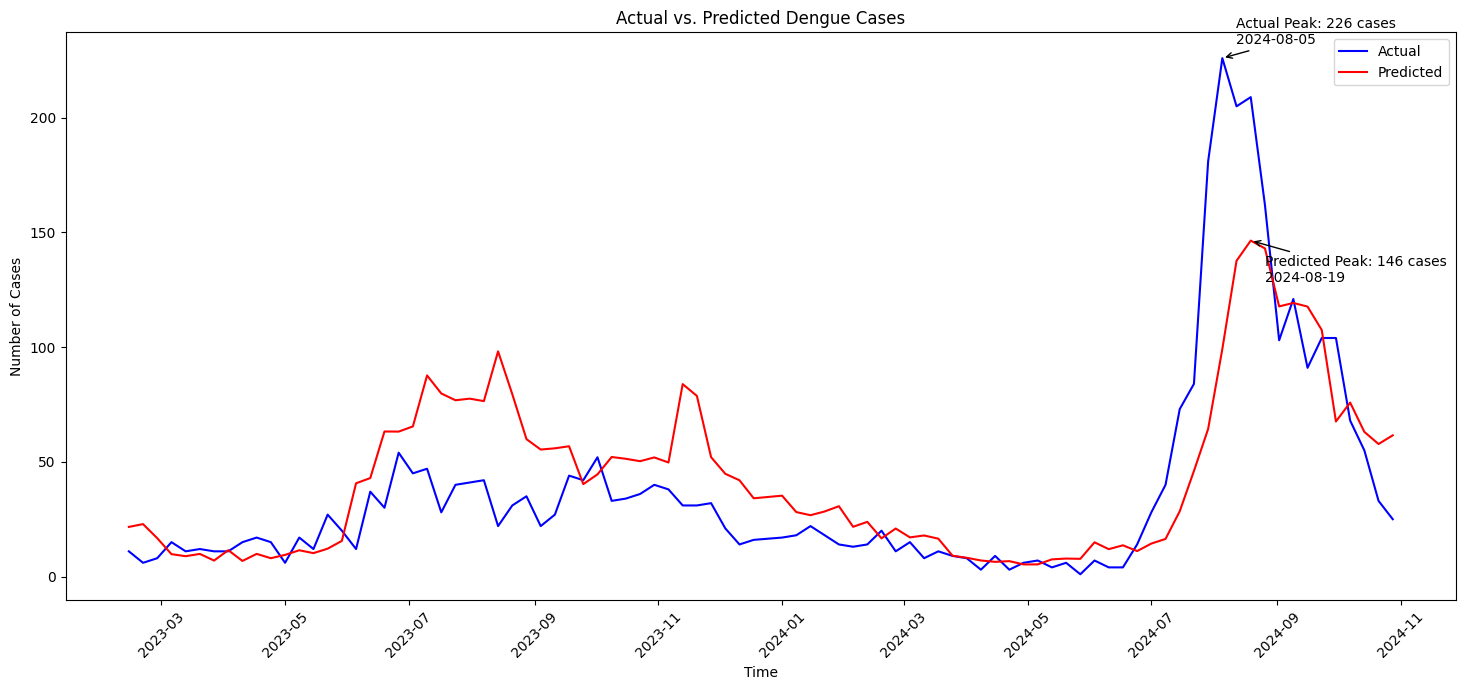
\includegraphics[width=1\linewidth]{image/Random Forest plot.png}
    \caption{Random Forest Actual vs Predicted}
    \label{fig:rf}
\end{figure}

In Figure \ref{fig:rf}. The plot illustrates that the Random Forest model effectively captures overall trends in dengue cases, particularly in the low to moderate ranges. However, it encounters challenges in accurately predicting peak values, often resulting in underestimations or overestimations. This indicates the model’s difficulty in handling high variability, leading to noticeable errors during periods of extreme fluctuations.\pagebreak

\begin{figure}[h!]
    \centering
    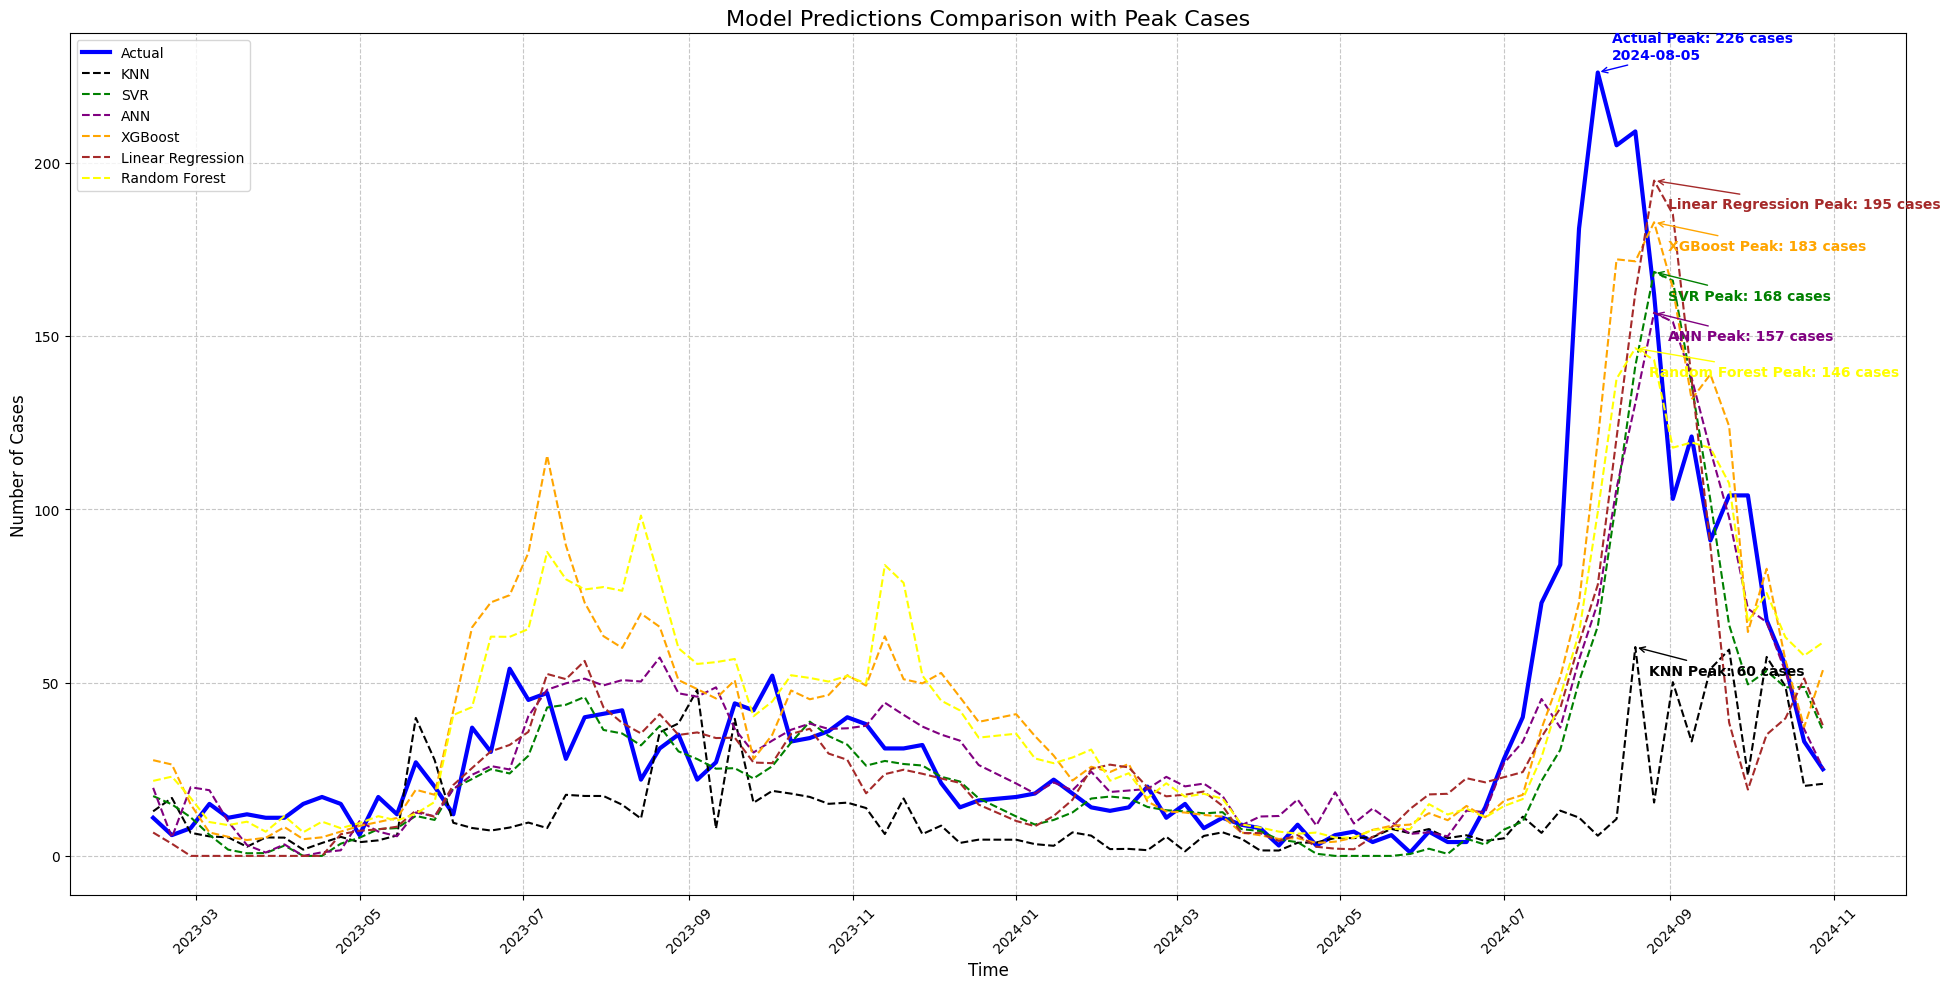
\includegraphics[width=1\linewidth]{image/All model plot.png}
    \caption{Plot of All Models}
    \label{fig:all}
\end{figure}

Figure \ref{fig:all} illustrates the comparative performance of the predictive models by plotting the predicted dengue cases generated by each model against the actual observed cases over the evaluation period. The visualization provides an in-depth perspective on how well each model captures the temporal trends and magnitude of dengue outbreaks, highlighting areas where predictions align closely with real data and instances of significant deviation.

\section{Conclusion}
Among the evaluated models, ANN demonstrated the lowest MAE (13.5304), indicating smaller average errors than other models, but its RMSE (27.3499), though low, was outperformed by Random Forest. The discrepancy between ANN's MSE and RMSE suggests it struggles with extreme values or outliers. Random Forest, on the other hand, achieved the lowest RMSE (25.4081) and MSE (645.5732), highlighting its ability to minimize overall errors and handle extreme variability effectively, despite having a slightly higher MAE than ANN. XGBoost performed better than most models but did not surpass ANN or Random Forest in any key metric. Meanwhile, SVR, Linear Regression, and KNN exhibited significantly higher RMSE and MAE values, making them less suitable for accurate dengue case forecasting.

Random Forest is the best-performing model based on RMSE and MSE, which are better indicators of overall predictive performance, especially for datasets with variability and outliers like dengue cases.
While ANN excels in minimizing average error (MAE), its higher RMSE and MSE compared to Random Forest suggest it is less robust in handling extreme cases.
Thus, Random Forest is recommended as the best model due to its superior generalization and error minimization across all ranges of dengue cases.

\bibliographystyle{apacite}  %-- specified APA style for bibliography
\bibliography{references}  %-- the file "myreferences.bib" contains the bibliography entries

\end{document}
